\section{Analysis} \label{secAnalysis}

With our results in hand, we now return to our seven questions we outlined in
section \ref{secMethod}.
Using our results we will answer each of them and comment on any insights we
have.

\subsection{Question one}

Originally, we wanted to know
\begin{quote}
  To what extent does learning carry over between two software projects of similar
  specifications?
\end{quote}
And, within our experimental framework we translated this to 
\begin{quote}
  What are the differences in $a$ between \PO\ using \LA\ and \PT\ using \LA?
\end{quote}

Our values for $a$ from our best fits for \PO\ using \LA\ and \PT\ using \LA are
shown in Tables \ref{table:P1LA:abc} and \ref{table:P2LA:abc} respectively.
We aggregate them and find that
\begin{itemize}
  \item the average of $a$ in \PO\ using \LA\ is 172.6738 minutes
  \item the standard deviation of our $a$ parameters in \PO\ using \LA\ is 0.23896 
  \item the average of $a$ in \PT\ using \LA\ is 100.0073 minutes
  \item the standard deviation of our $a$ parameters in \PT\ using \LA\ is
  0.068343
\end{itemize}

These low standard deviations suggests that these are very accurate estimates on
the amount of time a student takes to finish off a problem with no information
or knowledge about it.
This is sensible since the $a$ values were all very similar, and each model
should have started off with the same result for the first attempt at finishing
the problems.\\
\\
We note that between the \PO\ in \LA\ and \PT\ in \LA, there was a 72 minute
drop.
This is equivalent to a $42\%$ decrease in the required time to complete the
task, relative to the time taken in \PO\ in \LA.
It seems sensible that knowledge and time taken are inversely correlated.
Our results suggest that after completing a similar task, there is an increase of
$42\%$ in knowledge which is usable for this similar task.
Obviously, this is not entirely true --- there are differences in the tasks we
are using that we have not empirically considered.
Furthermore, we do not have a baseline of solving \PT\ without any prior
knowledge, but this gives an initial estimate on the increase of knowledge.

\subsection{Question two}

Our original question two asked
\begin{quote}
  To what extent does learning carry over between two software projects using
  similar resources?
\end{quote}

Within our experimental framework, this question asked
\begin{quote}
   What are the differences in $a$ between \PO\ using \LA\ and \PO\ using
  \LB?
\end{quote}

Again, we aggregate the $a$ values shown in Table \ref{table:P1LB:abc} and find
that
\begin{itemize}
  \item the average of the $a$ values of \PO\ using \LB\ is 102.9797 minutes
  \item the standard deviation of the $a$ values for \PO\ using \LB\ is 0.655761
\end{itemize}

The drop in $a$ values --- that is, the difference between the mean for \PO\
using \LA\ and \PO\ using \LB\ is very similar to what we found for Question
One.
Indeed, this is a 70 minute decrease, from the initial attempt in \PO\ in \LA\
to the first attempt for \PO\ in \LB.
This is a $40\%$ decrease compared to the $a$ value in \PO\ in \LA, and is quite
comparable to the decrease in the $a$ value in the previous section (\AZ\ of
\PO\ in \LA\ to \AZ\ of \PT\ in \LA).\\
\\
I had a personal suspicion that a language change would have a more significant
increase in knowledge and decrease in time than a change in problem
specification but our results suggest otherwise.
However, I do not think our results are conclusive and might actually support my
suspicions since prior to solving \PT, the students had actually completed \PO\
(a similar problem) problem eight times.
Conversely, when completing \PO\ in \LB\ they had only completed \PO\ four times.
This anomaly in process and experimental methodology suggests that
there is scope for more investigation and that my suspicions should not be
discarded yet.

\subsection{Question three}

Question three originally asks
\begin{quote}
  To what extent does practice enable us to better predict the effort required
  for software?
\end{quote}

This translates to us asking
\begin{quote}
  How well do our models fit the data?
\end{quote}

We want to know whether practice gives us better fits of models --- better fits
will suggest that our models are more useful for later predictions.
To answer this question, we will compare the sum of squares of the three
different datasets.
These are summarised in Tables \ref{table:P1LA:abc:sumsquares},
\ref{table:P1LB:abc:sumsquares} and \ref{table:P2LA:abc:sumsquares}.
We notice that \PO\ using \LA\ gives nonsensical results, and in fact our models
were inappropriate for actually doing much prediction (besides, perhaps $m_3$).
However, in \PT\ using \LA\ and \PO\ using \LB\ we retrieved sensible and useful
results.
\PO\ using \LB\ in particular had very good fits overall, with low sums of least
squares.\\
\\
I believe that this is due to actually practicing more on the same problem ---
we note that after performing the same problem (\PO) multiple times, even in
different languages, gives a more predictable result and is easier to fit a
model to.
Conversely, even though the problem is similar, the learning rate is much more
erratic and difficult to fit when completing \PT, despite using \LA.
This suggests that practicing on the same problem, regardless of language, will give more
consistent and predictable results for modelling purposes, whilst different
problems will cause issues with regards to being able to fit a model.

\subsection{Question four}

Our original question four asks
\begin{quote}
  How does learning differ as we practice on different problems? 
\end{quote}

We translate this, within the framework of our experiment to
\begin{quote}
   How does $b$ change between each of \PO\ in \LA, \PO\ in
   \LB\ and \PT\ in \LA?
\end{quote}

We re-summarise all the $b$ results from each dataset, for each model in Table
\ref{table:beees}.

\begin{table}[ht!]
\centering
\begin{tabular}{|c|c|c|c|}
\hline
  & $m_1$ & $m_2$ & $m_3$ \\
\hline
\PO\ in \LA & N/A & N/A & 0.794716 \\
\hline
\PO\ in \LB & 1.05646 & 1.05789 & 1.03095 \\
\hline
\PT\ in \LA & 1.78221 & 1.62075 & 1.39094 \\
\hline
\end{tabular}
\caption{These are the $b$ values from each fit. We omit the unreliable results
for $b$ in $m_1$ and $m_2$ for \PO\ in \LA.}
\label{table:beees}
\end{table}

There is an overall trend of $b$ increasing as the students do more iterations.
We ought to note that the $b$ value increasing makes the curve steeper, and it
reaches its horizontal asymptote (the value for $c$) much more quickly.
This suggests that reinforcement of knowledge through practice increases
learning and is an observable phenomena.\\
\\
An interesting question to ask is if the learning itself is asymptotic.
How much practice could we do before we would not increase learning anymore?
Figure \ref{fig:Bvaluefit} is a graph showing the means of the $b$ values and
the overall trend polynomial trend.

\begin{figure}[ht!]
\centering
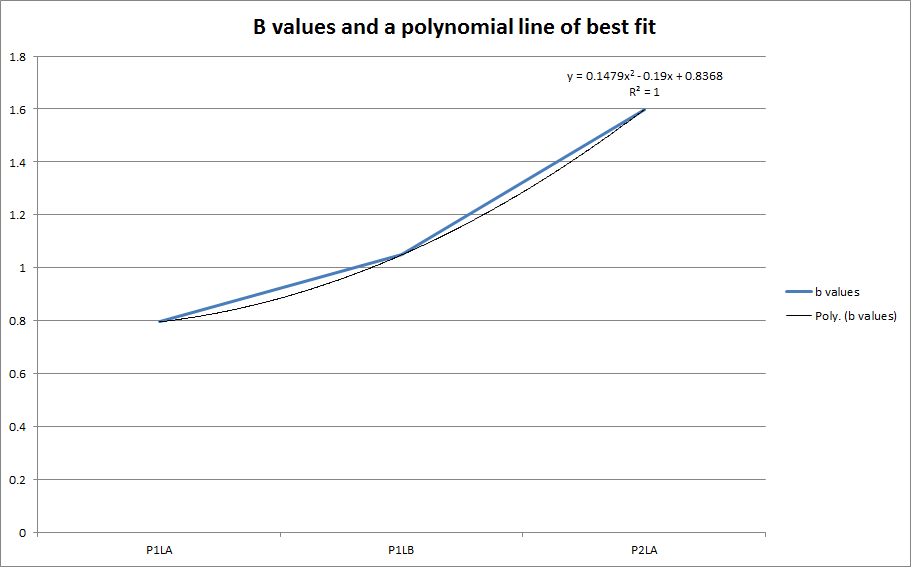
\includegraphics[scale=0.65]{./media/BValues.png}
\caption{The $b$-values after aggregation between each dataset.}
\label{fig:Bvaluefit}
\end{figure}

I think that we do not have enough data to make a conclusive comment about this,
but it is important to note that at present, the learning value apparently
is unbounded, and furthermore increases at an unbounded rate (by taking the
derivative of the equation of best fit).
This seems nonsensical to me, and I would suggest doing further analyses beyond
this rudimentary inspection to determine how learning changes and how learning
itself is affected between each iteration.

\subsection{Question five}

In question five, we wanted to explore how
\begin{quote}
  Prior research suggests that most of the time spent in making software is spent
  thinking --- if all the thinking has been performed, how long should it take to
  finish a project?
\end{quote}

Within our experiment, this meant examining
\begin{quote}
  What are the values for $c$ for each of \PO\ in \LA, \PO\ in \LB\ and \PT\ in
  \LA, and how reliable are these results?
\end{quote}

In Table \ref{table:CValues}, we show the aggregated $c$ values for each
dataset, omitting the negative $c$ values and showing the errors for these
calculations.

\begin{table}[ht!]
\centering
\begin{tabular}{|c|c|c|}
\hline
  {\bf Dataset} & {\bf Mean} & {\bf Error} \\
\hline
  \PO\ in \LA & 29.691 & 13.1391 \\
\hline
  \PO\ in \LB & 30.80703 & 1.20379 \\
\hline
  \PT\ in \LA & 35.67597 & 10.43677 \\
\hline
\end{tabular}
\caption{The aggregation of $c$ values for each dataset and the aggregation of
  the error. We note that ``error aggregation" is a poor method to use to
    analyse the errors and it could cause bias in our numbers.}
\label{table:CValues}
\end{table}

We do not include the $c$ values for \PO\ in \LA\ in our calculations.
Interestingly, the value for $c$ increases between each dataset, suggesting that
the effect of solving a problem with increased knowledge does not necessarily
translate to ending up with a lower time to completion overall.
We note that there was a much greater error for the third $c$ value (\PT\ in
\LA) than in the second $c$ value (\PO\ in \LB).\\
\\
This suggests that we had a very reliable result for the in analysing \PO\ in
\LB, whereas in the other results we had larger errors that reduce the
reliability of our results.
We also note as a caveat that the first $c$ value (\PO\ in \LA) is quite
unreliable due to us not having any other data points besides the fit of $m_3$
to use.

\subsection{Question six}

Question six originally asks
\begin{quote}
  How similar and consistent are the sizes of the solutions?
\end{quote}

Within our experimental framework this asks
\begin{quote}
  What is the variation in the lines of code of the solutions?
\end{quote}

We have shown the lines of code data in Table \ref{table:LOC} and Figure \ref{figure:LOC}.
It is clear that there is a high amount of variation between solutions in the
first few attempts, and that the drastically improve and start to converge to
around 98 lines of code.
The standard error of the lines of code was 60.80296.
We also took the coefficient of variation of the data, and found that it was
$0.455453$.
These two statistics together are indicative of the huge amounts of variation
that I showed in my solutions, and suggests that overall they were rather
dissimilar and inconsistent.\\
\\
I also tried fitting the three models to the data to see how if there were any
particular good fits.
We note that $m_3$ provides the best fit of the three models we use, which is
surprising since I would have expected $m_1$ and its relation to the Poisson
distribution to be more useful (where wastage or excess code is thought of as a
defect).
It is surprising that a simple factor, applied a number of times to the initial
number of lines of code is sufficient to model the changes in lines of code
effectively.

\subsection{Question seven}

Question seven asks
\begin{quote}
  Out of the theoretical models we have chosen, which is the best for modelling
  our process and why?
  Implicitly, we also ought to answer why the other models are inappropriate.
\end{quote}

I will make an argument that the best model to use for modelling is $m_3 =$
\[
  m_3(t) = (a-c) e^{-bt} + c
\]

We note that $m_3$ never had better results than $m_1$ or $m_2$ in terms of sum
of squares as a metric of how good a fit of a model was, except when being
fitted to my lines of code data.
However, $m_1$ and $m_2$ twice returned results that were hard to believe or
entirely nonsense, as shown in Tables \ref{table:P1LA:abc} and
\ref{table:mytimes:abc}.
Although they ($m_1$ and $m_2$) present better fits for most time-based data, I believe these are
glaring weaknesses in these models and that they are not as robust or
appropriate for modelling as $m_3$.\\
\\
However, we ought to note that we only used four data points and this would have
made it difficult to fit the model accurately.
Perhaps with more data, $m_1$ and $m_2$ would have behaved more sensibly and
would have not yielded negative values.
Even so, I believe we should also note that in software engineering, it might be
difficult to obtain lots of data, and a model should be tolerant to yielding
nonsense values, which $m_1$ and $m_2$ are not.
Therefore, I would advocate discarding them for modelling purposes and using
$m_3$ as the most appropriate model for modelling purposes.
